
\documentclass[a4paper, 12pt]{article}
\usepackage{graphicx}

\usepackage[utf8]{inputenc}
\usepackage[magyar]{babel}

% a szép matematikai szimbólumokért
\usepackage{amssymb}
\usepackage{amsmath}

% ha táblázatban szeretnénk egyesített sorokat is
\usepackage{multirow}

% horizontal line
\usepackage{hhline}

% eps formátumú ábrák --> pdflatex fordításhoz!!
\usepackage{epsfig}

% egyenletekhez, pl mátrixok írására
\usepackage{array}

% ha betűszíneket is szeretnénk használni
\usepackage{color}

% Margók egyéni beállításai
\usepackage{anysize}
\marginsize{1.64cm}{1.64cm}{1.2cm}{2.4cm} %\left right top bottom

% vakszöveg
\usepackage{lipsum}
\usepackage{blindtext}

% A HIVATKOZÁSOKHOZ HASZNÁLT CSOMAGOK. RÉSZLETESEBBEN LD: google -> latex bibtex
\usepackage[numbers, square, comma, sort&compress]{natbib}
%\usepackage[format=hang,labelsep=period]{caption}

\usepackage[unicode]{hyperref}   % ezzel a hivatkozások linkké válnak
\usepackage{bookmark}
\hypersetup{bookmarksopen={true}}
\hypersetup{bookmarksopenlevel={2}}
\hypersetup{bookmarksnumbered={true}}
\hypersetup{
  colorlinks,%
  citecolor=red,%
  filecolor=black,%                                                                                                                                               
  linkcolor=blue,%
  urlcolor=green
}
\numberwithin{equation}{section}          % ezekkel tudod beállítani, hogy milyen felbontásig menjen a hivatkozás
\numberwithin{figure}{subsection}
%\numberwithin{table}{section}          % ha kikommenteled, akkor csak simán számozva lesz.

%%%%%%%%%%%%%%%% Néhány dolog a fancy kinézethez

\frenchspacing
\setlength{\parskip}{2ex}
\setlength{\headsep}{0,4cm}
\setlength{\headheight}{4pt}

% fej- es lábléc
\usepackage{fancyhdr}
\usepackage{fancyref}
\usepackage{fancyvrb}
\pagestyle{empty}

\renewcommand{\headrulewidth}{0,05pt}
\renewcommand{\footrulewidth}{0pt}


\fancyhf{}
\fancyhead[RE]{{ \nouppercase{\leftmark}} }
\fancyhead[LO]{{ \nouppercase{\leftmark}} }
\cfoot{--~\thepage~--}


%%%%%%%%%%%%%%%%%%%%%%%%%%%


%%%%%%%%%%%%%%%%%%%%%%%%%%%%%%%%%%%%%%%%%%%%%%%%%%%%%%%%%%%%%%%%%%%%%%%%%%%%

\begin{document}

% Címoldalt lehet egyszerűen a \maketitle paranccsal is. Ha kissé részletesebb
% címre van szükség, azt lehet így is, kézzel megadva mindent.
\begin{titlepage}   
\begin{center}
\thispagestyle{empty}  

\vspace*{0.7cm}
\rule{\linewidth}{0.5mm} \\[3mm]
\vspace*{0.7cm}

{\LARGE Szintvonalak meghatározása a marching squares algoritmusssal}

\vspace*{0.7cm}
\rule{\linewidth}{0.5mm} \\[3mm]
\rule{\linewidth}{0.5mm} \\[3mm]



{\Large Programleírás\\}

\vspace*{0.7cm}
\rule{\linewidth}{0.5mm} \\[3mm]
  {\small Beadandó} \\[3mm]
  \vspace*{1cm}
{\footnotesize Írta: Csabai Bence} \\
{\tiny csabai.bence@gmail.com}

  \vspace*{1cm}

\begin{figure}[h!]
\begin{center}

\includegraphics[width=0.5\textwidth]{img/elte}
\end{center}
\end{figure}

\end{center}
\end{titlepage}

\newpage



\thispagestyle{empty}  

\begin{abstract}
  A program amelyet készítettem egy domborzati térkép szintvonalainak meghatározására való. Ahhoz, hogy ezt elérjem, az úgynevezett \textit{marching squares} módszert módszert implementáltam a programba. Emellett a program képes megmondani egy pontról, hogy belül van-e egy adott szintvonalon. Ezt a \textit{winding number} nevű technikával állapítom meg.


\end{abstract}


\newpage \vspace*{2cm}
\thispagestyle{plain}                                                                                                                                             
\pagenumbering{roman} \setcounter{page}{1}
\tableofcontents

\newpage \vspace*{2cm}
\thispagestyle{plain}
\listoffigures
\endLOFtrue

\newpage \vspace*{2cm}

\pagenumbering{arabic} \setcounter{page}{1}
\pagestyle{empty}



\section{Bevezetés}
\label{sec:bev}
A szintvonalak meghatározása fontos feladat, mivel ezek sok értéket képviselnek az élet több területén is. Természetesen elsősorban amikor a szintvonalakra gondolunk, a turistatérképek jutnak eszünkbe: jelzik az utazónak melyik ösvény a meredekebb (a vonalak sűrűbben vannak) illetve melyik lankásabb (a vonalak ritkábbak). De emellett gondolhatunk a 3D-s képek megjelenítésére vagy akár hőmérséklet és széltérképekre. A program ezt a problémát oldja meg. 


\section{Elvi működés}
\label{sec:fejezet}

Alábbiakban leírom a program elvi és technikai működését
\subsection{Beolvasás és előkészítés}
\label{subsec:alfejezet}

Mielőtt a programunk elkezdheti végezni a fő feladatát szükségünk van jól előkészített adatokra. Ezeket az adatokat megfelelő módon be kell olvasni és preparálnunk kell az adatokat, melyeken a kontúrvonalakra kíváncsiak vagyunk.

\subsubsection{Beolvasás}
\label{subsubsec:alalfejezet}

A programot természetesen az adatok beolvasásával kezdjük. Az adatok egy fileban vannak, ennek megyek végig sorain hogy a programom tudja használni a benne lévő adatokat. Fontos, hogy a fájl csak valós számokat tartalmazzon egy n*k-s formátumban, különben a beolvasás lehetetlen lesz

\subsubsection{Adatelőkészítés}
\label{subsubsec:alalfejezet2}

A ....ban leírt marching squares algoritmus eredetileg nem valós számokra, hanem 0-kra és 1-ekre működik csak, éppen ezért a beolvasott adatokat ilyen formára kell fordítanunk. Ehhez egy függvényt írtam, mely egy adott adathalmazban megvizsgálja, hogy egy elem nagyobb-e mint az előre meghatározott határ. Ha igen, egy új, az eredetivel megegyező méretű táblában erre a helyre 1-est, ha pedig nem, akkor 0-st ír.  


\subsection{Marching Squares}

A marching squares egy számítógépes grafikai algoritmus amu kontúrokat generál egy két dimenziós skalármezőhöz (téglalap alakú tömbje különálló számoknak) \cite{wiki1} Az eljárás lényege, hogy a korábban 0/1-essé alakított adatokon végigmegy, és megvizsgálja az összes pontnégyest, ahogy a \ref{fig:lookup} ábrán látható.

\begin{figure}[h!]
\begin{center}
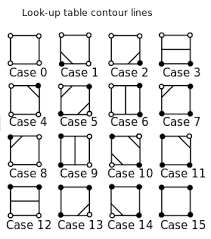
\includegraphics[width=0.5\textwidth]{img/download.png}
\caption{Kontúr vonal esetek}
\label{fig:lookup}
\end{center}
\end{figure}

Ezeknek 16 különböző kombinációjuk van, így ezt megfigyelve tudja eldönteni a módszer, hogy melyik élet kell berajzolnia. Egyszerűen ez úgy volt leprogramozható, hogy vesszük sorban a sarkokat, és mindegyiknek értékét beszorozzuk egy kettőhatvánnyal, majd ezeket összeadjuk: 

\begin{equation}
    val=8a_1+4\cdot a_2+2\cdot a_4+1\cdot a_3
\end{equation}

Így minden kombinációra egyedi érték jön ki. Ha erre írunk egy függvényt, kapunk egy $(n-1)\times(k-1)$ méretű mátrixot, ahol már az adott szintvonal be van jelölve az elemek értéke által.

\newpage
Ezután a 15-ösöket 0-sra cserélve (lényegük ugyan az, vonal nem rajzolódik) és több szintvonal mátrixot összeadva, kaphatunk egy kész térképet, amin már több szintvonal is be van jelölve. A \ref{fig:cont} ábrán a különböző árnyalatú pixelek a 15 esetet reprezentálják. 

\begin{figure}[h!]
\begin{center}
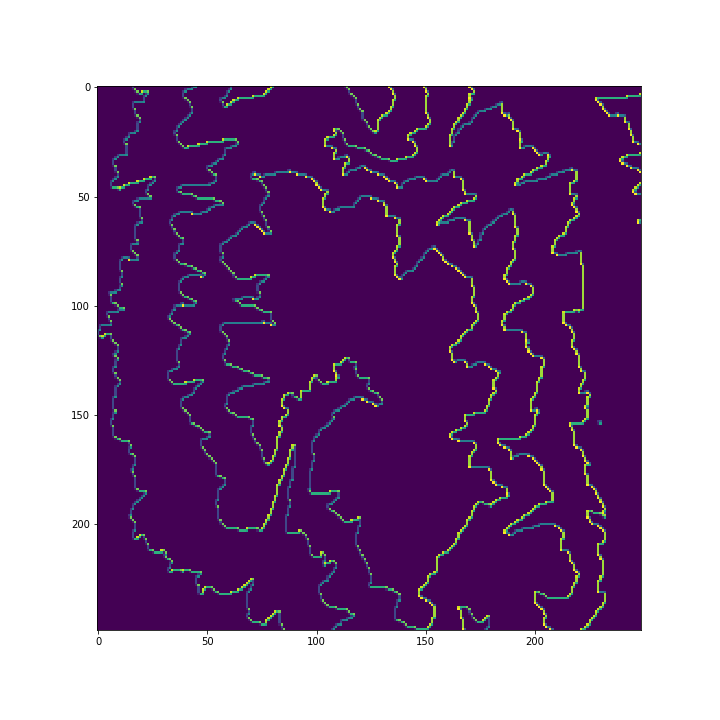
\includegraphics[width=0.5\textwidth]{img/cont.png}
\caption{Kontúrok a Hargita hegységben}
\label{fig:cont}
\end{center}
\end{figure}



\subsection{Winding Number}

Végső featureként a program a winding number nevű technikát használva meg tudja állapítani egy adott pontról, hogy egy adott kontúron belül van-e. A metódus lényege, hogy összekötjük a pontunk a kontúr egy pontjával, körbehaladunk a kontúrvonalon és mérjük a szöget. Amennyiben körbeérünk és a pont a kontúron belül van, a szög $2\pi$ lesz.



\newpage \vspace*{2cm}

\pagestyle{empty}

\begin{thebibliography}{9}
\bibitem{wiki1} 
Wikipedia 
\textit{Marching squares}. 
\\\texttt{https://en.wikipedia.org/wiki/Marching_squares}

\end{thebibliography}


\end{document}

© 2019 GitHub, Inc.
Terms
Privacy
Security
Status
Help
Contact GitHub
Pricing
API
Training
Blog
About
